
\begin{frame}{Reactive walking pattern generation \only<4>{with obstacles}}
\framesubtitle{
  \textcolor{green!30!black!80}
  {
    (M. Naveau, RA-L 2016) ; 
    (M. Naveau, Humanoids 2014)
  }
}

  \begin{minipage}{0.48\textwidth}
  \vspace*{0.2cm}
    Optimization problem solved:
    \vspace*{-0.3cm}
    \only<1-3>{
        \begin{equation*}
          \begin{aligned}
            \min_{{\bf U}_k} 
            \sum_{i=0}^{j=4} w_i J_i({\bf U}_{k}) & \\
                {\bf X}_{k+1} = {\bf A}{\bf X}_{k} + {\bf C} {\bf U}_k & \\
                \underline{\bf P} < {\bf P} {\bf U}_k  < \overline{\bf P}& \\
          \end{aligned}
        \end{equation*}
        with ${\bf U}_k=\begin{pmatrix} \dddot{\bf X}_k \; {\bf X}_k^\mathit{f}\; \dddot{\bf Y}_k \;{\bf Y}_k^\mathit{f}  \end{pmatrix}^T$ \\        
      }
      \only<4>{
        \begin{equation*}
          \begin{aligned}
            \min_{{\bf U}_k} 
            \sum_{i=0}^{j=4} w_i J_i({\bf U}_{k}) & \\
                {\bf X}_{k+1} = {\bf A}{\bf X}_{k} + {\bf C} {\bf U}_k & \\
                \underline{\bf P} < {\bf P}{\color{red}{({\bf U}_k)}} {\bf U}_k  < \overline{\bf P}& \\
          \end{aligned}
        \end{equation*}
      with ${\bf U}_k=\begin{pmatrix} \dddot{\bf X}_k \; {\bf X}_k^\mathit{f}\; \dddot{\bf Y}_k \;{\bf Y}_k^\mathit{f} \;\color{red}{{\bf \Theta}_k^\mathit{f}}\end{pmatrix}^T$ \\
      }
  \end{minipage}
  %
  \begin{minipage}{0.48\textwidth}
    \only<1-3>{
      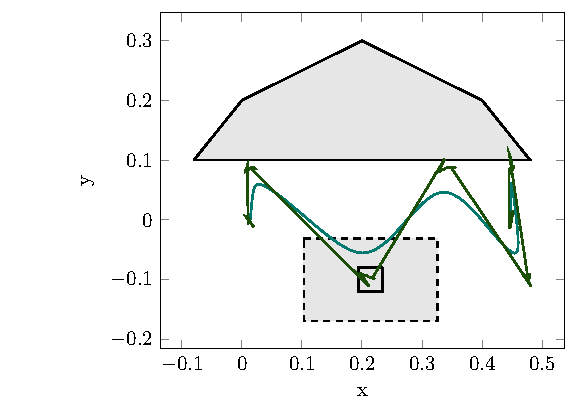
\includegraphics[width=\textwidth]{./images/tikz/convexHulls2}
    }
    \only<4>{
      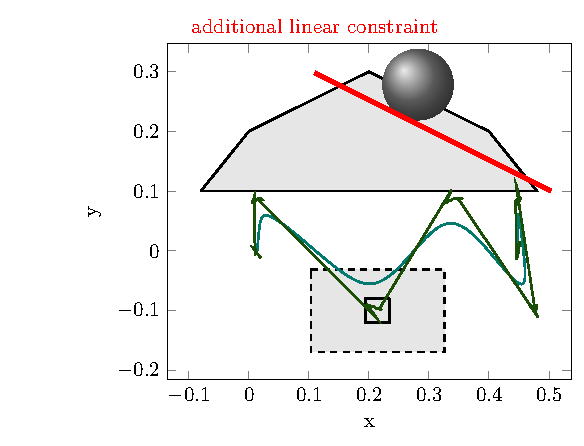
\includegraphics[width=\textwidth]{./images/tikz/convexHullsplusObstacles2}
    }
  \end{minipage}\\

  \only<1>{
    $J_1({\bf U}_{k})$ is the linear velocity tracking 
    {\small
      \begin{equation*}
        J_1({\bf U}_k) = \lVert \dot {\bf X}_{k} - {\bf X}_{k}^{ref} \rVert^2_2
        +  \lVert \dot {\bf Y}_{k} - {\bf Y}_{k}^{ref} \rVert^2_2 
      \end{equation*}}
    }
    \only<2>{$J_2({\bf U}_{k})$ is the control norm
      {\small
        \begin{equation*}
          J_2({\bf U}_k) = \lVert \dddot {\bf X}_{k} \rVert^2_2
          + \lVert \dddot {\bf Y}_{k} \rVert^2_2
        \end{equation*}
      }
    }
    \only<3>{$J_3({\bf U}_{k})$ is distance of the CoP to the most stable trajectory
      {\small
        \begin{equation*}
          J_3({\bf U}_k) = \lVert {\bf X}_{k}^{f} - CoP_{k+1}^{x} \rVert^2_2 +
          \lVert {\bf Y}_{k+1}^{f} - CoP_{k+1}^{y} \rVert^2_2 
        \end{equation*}
      }
    }
    \only<4>{$J_4({\bf U}_{k})$ is the angular velocity tracking
      {\small
        \begin{equation*}
            J_4({\bf U}_k) = \lVert {\bf \Theta}_{k} 
            - \int {\bf \Theta}_{k}^{ref} dt \; \rVert_2^2 
        \end{equation*}}
    }    

\end{frame}

%%%%%%%%%%%%%%%%%%%%%%%%%%%%%%%%%%%%%%%%%%%%%%%%%%%%%%%%%%%%%%%%%%%%%%%%%%%%%%%


\begin{frame}{Solver}

\begin{itemize}
\item Original nonlinear problem :
  \begin{align*}
    \min_{\color{txtcolor2}{\bf U}_k}  \quad & J({\color{txtcolor2}{\bf U}_k}) \\
    \text{s.t.} \quad & \underline{\bf P} \leq \tilde{\bf P}({\color{txtcolor2}{\bf U}_k}) \leq \overline{\bf P}
  \end{align*}
\item QP approximation :
  \begin{align*}
    \min_{{\color{txtcolor5}{\bf \Delta U}_k}} \quad &
    Grad(J)({\bf U}_{k-1}) {\color{txtcolor5}{\bf \Delta U}_k} +
    \frac{1}{2} {\color{txtcolor5}{\bf \Delta U}_k}^T Hess(J)({\bf U}_{k-1}) {\color{txtcolor5}{\bf \Delta U}_k} \\
    \text{s.t.} \quad & \underline{h} - h_{k-1} \leq Jac(\tilde{\bf P})({\bf U}_{k-1}) {\color{txtcolor5}{\bf \Delta U}_k} \leq \overline{h} - h_{k-1}\\
    {\color{txtcolor2}{\bf U}_k} =& {\bf U}_{k-1} + \alpha {\color{txtcolor5}{\bf \Delta U}_k}
  \end{align*}
\end{itemize}
\end{frame}

%%%%%%%%%%%%%%%%%%%%%%%%%%%%%%%%%%%%%%%%%%%%%%%%%%%%%%%%%%%%%%%%%%%%%%%%%%%%%%%

\begin{frame}{Walking without thinking}

\begin{center}
  \hspace*{-1cm}
  \scalebox{0.7}{%!TEX root = ../../14-icra-RealTimeNMPC.tex

\tikzstyle{block} = [draw, fill=blue!20, rectangle,
    minimum height=2em, minimum width=5em, align=center]
\tikzstyle{sum} = [draw, fill=blue!20, circle, node distance=1cm]
\tikzstyle{input} = [coordinate]
\tikzstyle{output} = [coordinate]
\tikzstyle{pinstyle} = [pin edge={to-,thin,black}]

% The block diagram code is probably more verbose than necessary
\begin{tikzpicture}[auto, node distance=2cm,>=latex]

    % We start by placing the blocks
    \node [input]  at (0.0, 0.0) (input)  {};
    \node [input]  at (3, 0.0) (velocity) {};
    \node [input]  at (7.2, -2.8) (feedback)  {};
    \node [input]  at (16, -2.8) (feedback2)  {};
    \node []    at ( 0.0, 0.0) (sumin)  {};
    %\node [output]    at ( 15, 0.0) (sumout) {};
    \draw [fill=green,opacity=.2,text opacity=1] (0.1,1.5) rectangle (12.6,-2.0);
    \node at(10,-1.7) {\textcolor{green!20!black!100}{Stack of Tasks}};

%    \node [block] at (4.6,-1.7) (lwc) {
%        Left Wrist\\
%        Hybrid\\
%        Controller        
%    };

%    \node [block] at (1.7,0.0) (walking) {
%        Walking \\
%        Task    
%    };

    \node [block] at (1.7,0) (wpg) {
        Walking\\
        Pattern\\
        Generator
    };
    \node [block, fill=green!30!black!80] at (5.2,0) (dyn) {
        Dynamic\\
        Filter
    };
    \node [block] at (8.5,0) (ttt) {
        Task for\\
        Trajectory\\
        Tracking
    };    
    \node [block] at (11.5,0) (qp) {
        HQP\\
        solver
    };
    \node [block] at (15, 0) (system) {
    		Robot Hardware\\
    		{\footnotesize Simulation/Robot}\\
    		and\\
    		{\footnotesize motion capture system}
    	};

    % PATHS
    	% Forward chaine
%    \draw [draw,-] (input) -- node {\small ${\mathbf{p}}^{\,{\text {ref}}}$} (walking);
    
    \draw [draw,->] ([xshift=-2cm]wpg.west) -- node {\small ${\mathbf v}^{\,{\text{ref}}}$} (wpg);
%    \draw [draw,- ] (walking) -- node {} (velocity);
%    \draw [draw,->] (velocity) |- node {} (lwc);
%    \draw [->] (wpg) -- node {\small $c^{ref},f^{ref}$} (dyn);
%    \draw [->] (dyn) -- node {\small $\tilde{c}^{\,ref},f^{ref}$} (sot);
    \draw [->] (wpg) -- node [text width=1cm]{\small ${\mathbf{p}_{com}}^{\,{\text {ref}}}$ ${\mathbf{p}_{foot}}^{\,{\text {ref}}}$} (dyn);
    
    \draw [->] (dyn) -- node [text width=1cm]{\small ${\tilde{\mathbf{p}}_{com}}^{\,{\text {ref}}}$ ${\mathbf{p}_{foot}}^{\,{\text {ref}}}$} (ttt);
    
    \draw [->] (ttt) -- node [text width=1cm]{
    \small Tasks
    } (qp);
    \draw [->] (qp) -- node [text width=0.6cm]{\small ${\mathbf q}^{\,{\text{ref}}}$ $\dot{{\mathbf q}}^{\,{\text{ref}}}$} (system);
    
%    \draw [->] (lwc) -| node [near start, above]{\small ${\mathbf{p}_{lw}}^{\,{\text {ref}}}$} (ttt);
    %\draw [->] (system) -- node {} (sumout);

    % Feedback chaine
    \draw [- ] ([xshift=+0.8cm]dyn.east) |- node {}
               ([xshift=-0.5cm,yshift=-1.0cm]wpg.west);
    \draw [->] ([xshift=-0.5cm,yshift=-1.0cm]wpg.west) |- node {}
               ([yshift=-0.2cm]wpg.west);
    
%    \draw [- ] (system.east)    -| node {} (feedback2);
%    \draw [- ] (feedback2)  -- node [above]{\small $\mathbf{f}_{lw},\mathbf{p}_{w},\mathbf{p}_{lw},\mathbf{p}_{f}$} (feedback);
%    \draw [->] (3.0,-2.8) |- node [near start, above]{} ([yshift=-0.2cm]lwc.west);
%    \draw [->] (feedback) |- node [below=0.7cm, right]{\small $\mathbf{p}_{ch}$} ([yshift=-0.2cm]walking);

%    \draw [->] (dyn) -| node[above right] {\small $\hat{c}^{\,x,y,\theta}$, $\hat{f}^{\,\,x,y,\theta}$} (wpg);
\end{tikzpicture}
}
\end{center}

\end{frame}

%%%%%%%%%%%%%%%%%%%%%%%%%%%%%%%%%%%%%%%%%%%%%%%%%%%%%%%%%%%%%%%%%%%%%%%%%%%%%%%

\begin{frame}{Experiment on HRP2}
  \begin{center}
    \movie[autostart,loop]{
    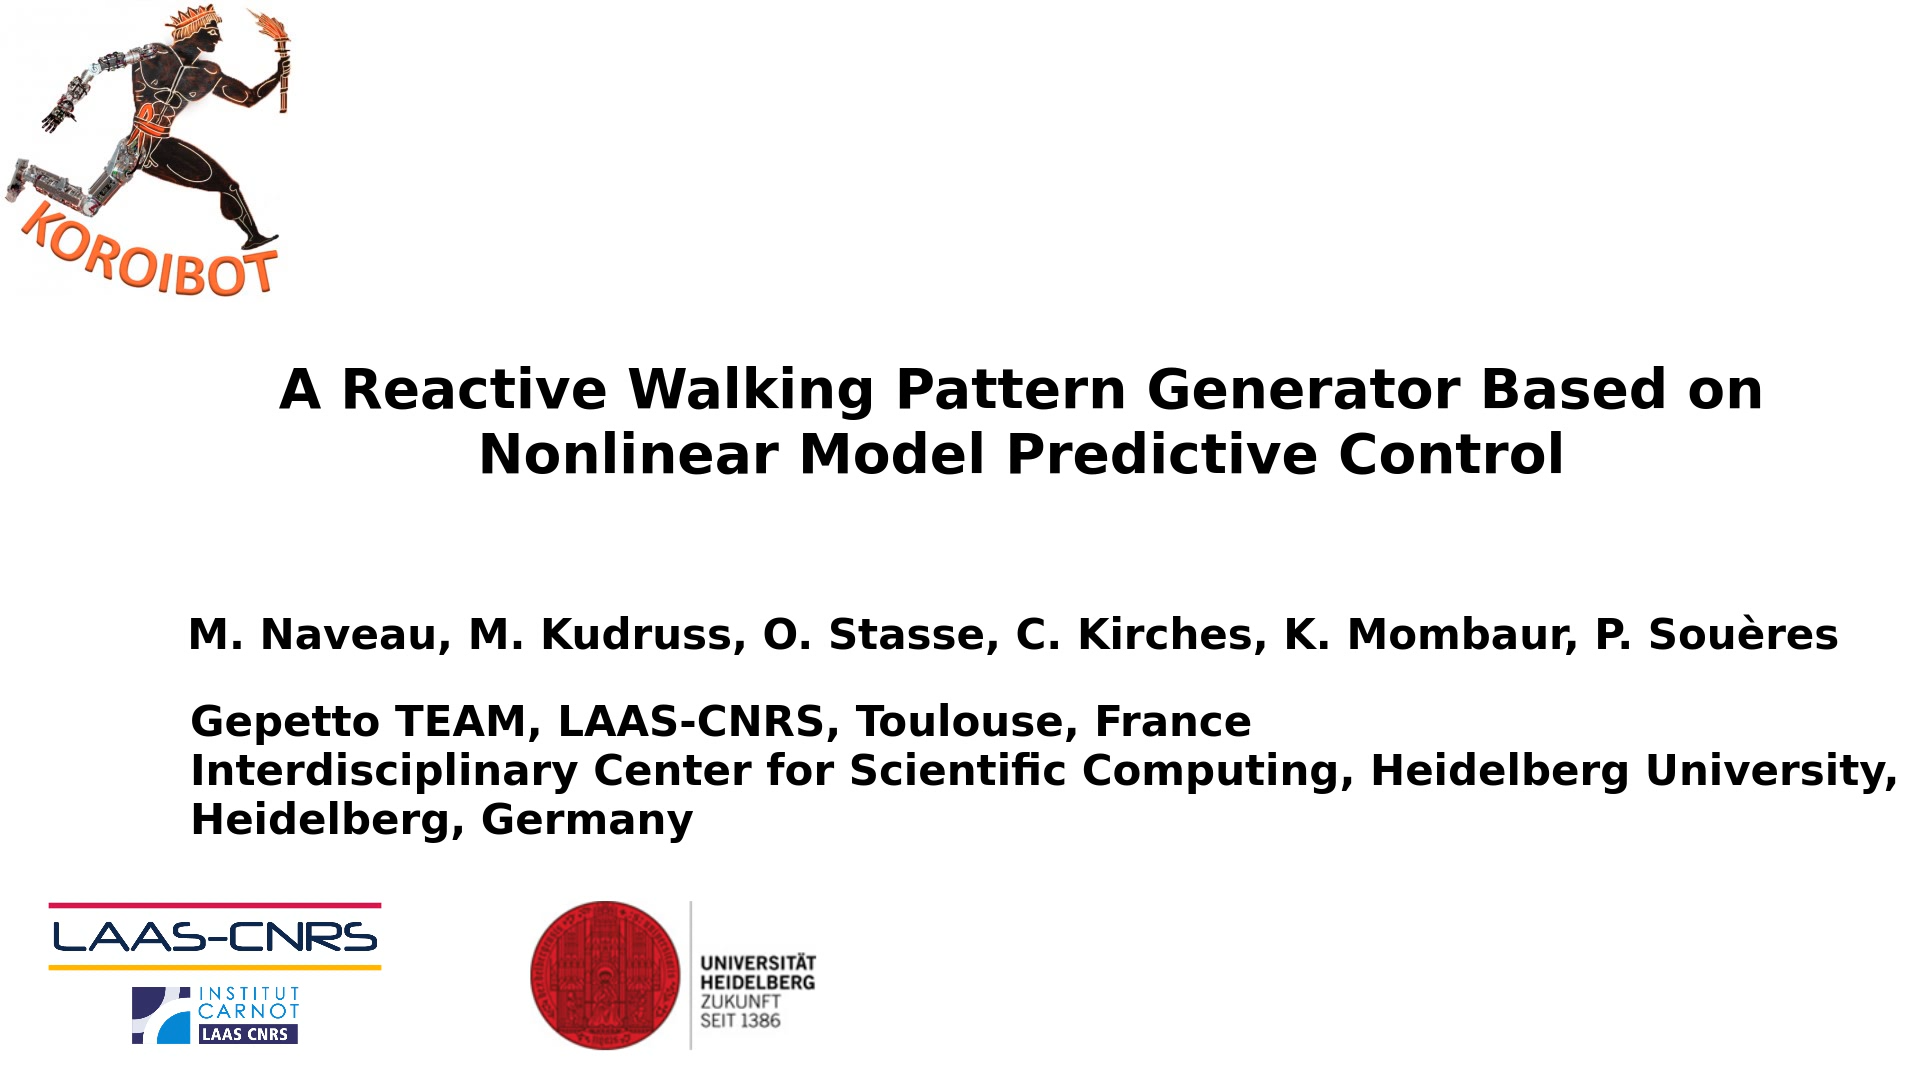
\includegraphics[width=0.85\linewidth, keepaspectratio]
      {16-raletter-NMPC-v19.png}    
    }  
    {videos/16-raletter-NMPC-v19.mp4}
  \end{center}
\end{frame}

%%%%%%%%%%%%%%%%%%%%%%%%%%%%%%%%%%%%%%%%%%%%%%%%%%%%%%%%%%%%%%%%%%%%%%%%%%%%%%%

